\documentclass[conference]{IEEEtran}
\usepackage[utf8]{inputenc}
\usepackage[T1]{fontenc}
\usepackage[french]{babel}
\usepackage{amsmath,amssymb}
\usepackage{graphicx}
\usepackage{booktabs}
\usepackage{tikz}
\usetikzlibrary{arrows.meta,positioning,shapes.geometric,shapes.multipart,fit,calc}
\usepackage[hidelinks]{hyperref}



\begin{document}

\title{Algorithme d'\'Evolution Diff\'erentielle massivement parall\`ele sur GPU avec CUDA : comparaison avec la version s\'equentielle}

\author{
  \IEEEauthorblockN{Zainab Elamri, Omar Elsemry, Mohamed De Franceschi}
  \IEEEauthorblockA{Master IM -- Universit\'e de Haute-Alsace (UHA)\\
  Enseignant : Lhassane IDOUMGHAR}
}

\maketitle

\begin{abstract}
Nous \'etudions la parall\'elisation massive sur GPU de l'\'Evolution Diff\'erentielle (DE/rand/1/bin) \`a partir d'un code CUDA de PSO fourni par l'enseignant. Nous en d\'erivons une version s\'equentielle (CPU) et une version GPU o\`u chaque thread traite un individu, puis nous les comparons au PSO d'origine sur quatre fonctions de test (Sphere, Rastrigin, Rosenbrock, Griewank d\'ecal\'ees), pour $\mathrm{Dim}\in\{10,50,100\}$, $\mathrm{Pop}\in\{50,100,500\}$ et un budget de $10^4\times\mathrm{Dim}$ \'evaluations. Sur une NVIDIA RTX 2080 Ti, le DE GPU est jusqu'\`a 27 fois plus rapide que le DE s\'equentiel (m\'ediane 3,5), pour une qualit\'e statistiquement \'equivalente dans 34 configurations sur 36, et il surpasse significativement le PSO de r\'ef\'erence dans 34 configurations sur 36. Nous comparons aussi les taux de succ\`es \`a ceux publi\'es pour cudaDEi \cite{qin}, en testant le param\`etre $CR=0{,}3$ de cet article, qui am\'eliore les grandes populations mais d\'et\'eriore Rosenbrock, et nous discutons les limites li\'ees \`a la simple pr\'ecision.
\end{abstract}

\begin{IEEEkeywords}
Differential Evolution, GPU, CUDA, massively parallel metaheuristics, global optimization, benchmark functions.
\end{IEEEkeywords}

%--------------------------------------------------------------
\section{Introduction}
Beaucoup de probl\`emes d'ing\'enierie se ram\`enent \`a la recherche d'un minimum global $x^\star=\arg\min_{x\in[x_{\min},x_{\max}]^D} f(x)$ d'une fonction non convexe, pour laquelle les m\'ethodes \`a gradient sont inop\'erantes. Les m\'etaheuristiques de population, comme l'optimisation par essaims particulaires (PSO) et l'\'evolution diff\'erentielle (DE) \cite{storn}, sont des alternatives courantes, mais leur co\^ut croît avec la dimension et la taille de la population.

Ces algorithmes sont naturellement parall\`eles : les individus subissent les m\^emes op\'erations, et les GPU, qui ex\'ecutent des milliers de threads, s'y pr\^etent bien \cite{qin}. L'objectif de ce travail de Master est d'\'etudier une version massivement parall\`ele du PSO fournie en CUDA, de la transformer en DE, et de comparer le r\'esultat \`a une version s\'equentielle et \`a la litt\'erature.

Nos contributions sont : (i) une impl\'ementation s\'equentielle et une impl\'ementation GPU (un thread par individu) de DE/rand/1/bin, (ii) un protocole exp\'erimental reproductible (10 runs, 3 dimensions, 3 tailles de population, 4 fonctions), (iii) une comparaison avec le PSO de r\'ef\'erence et, pour la qualit\'e, avec cudaDEi \cite{qin}. La section~II rappelle la programmation GPU, la section~III d\'ecrit le DE et nos impl\'ementations, la section~IV pr\'esente les r\'esultats et la section~V conclut.

%--------------------------------------------------------------
\section{Programmation GPU}
CUDA est la plateforme de calcul parall\`ele de NVIDIA. Le programme est h\'et\'erog\`ene : le code \emph{h\^ote} (CPU) alloue la m\'emoire, copie les donn\'ees et lance des \emph{noyaux} (\texttt{\_\_global\_\_}) qui s'ex\'ecutent sur le \emph{device} (GPU). Un lancement \texttt{kernel<<<blocs, threads>>>} cr\'ee une grille de blocs de threads ; les threads d'un bloc sont ex\'ecut\'es par groupes de 32 (\emph{warps}) sur un multiprocesseur (SM) selon le mod\`ele SIMT. Les fonctions \texttt{\_\_device\_\_} ne sont appelables que depuis le GPU.

La m\'emoire est hi\'erarchis\'ee : registres et m\'emoire locale par thread, m\'emoire partag\'ee par bloc (rapide), m\'emoire globale accessible \`a tous mais de latence \'elev\'ee. Les transferts h\^ote$\leftrightarrow$device passent par le bus PCIe et sont co\^uteux : une bonne impl\'ementation les minimise. Pour le g\'en\'erateur al\'eatoire, la biblioth\`eque cuRAND fournit un \'etat (\texttt{curandState}) par thread.

Nos mesures ont \'et\'e faites sur une NVIDIA GeForce RTX 2080 Ti (architecture Turing, capacit\'e de calcul 7.5, 11~Go) avec CUDA~13.4, compil\'e pour \texttt{sm\_75}.

%--------------------------------------------------------------
\section{\'Evolution Diff\'erentielle}

\subsection{Aper\c cu de la version s\'equentielle}
La DE \cite{storn} fait \'evoluer une population de $N_P$ vecteurs $x_i\in\mathbb{R}^D$ tir\'es uniform\'ement dans $[-5{,}12;\,5{,}12]^D$. \`A chaque g\'en\'eration, pour chaque individu $x_i$ (le \emph{vecteur cible}) :
\begin{enumerate}
\item \textbf{Mutation} : on tire trois indices distincts $r_1,r_2,r_3\neq i$ et on forme $v_i=x_{r_1}+F\,(x_{r_2}-x_{r_3})$.
\item \textbf{Croisement binomial} : $u_{i,j}=v_{i,j}$ si $\mathrm{rand}_j<CR$ ou $j=j_{\mathrm{rand}}$, sinon $u_{i,j}=x_{i,j}$ ; $j_{\mathrm{rand}}$ garantit qu'au moins une composante vient du mutant. Le r\'esultat est ramen\'e dans les bornes.
\item \textbf{S\'election} : $x_i\leftarrow u_i$ si $f(u_i)\le f(x_i)$, sinon $x_i$ est conserv\'e.
\end{enumerate}
Nous utilisons $F=0{,}5$ et, selon la s\'erie d'exp\'eriences, $CR=0{,}9$ ou $CR=0{,}3$ (valeur de l'article \cite{qin}). Les lectures se font dans la population de la g\'en\'eration $g$ et les \'ecritures dans celle de $g{+}1$ (double buffer), ce qui rend les individus ind\'ependants au sein d'une g\'en\'eration. Le nombre de g\'en\'erations est $G=10^4\times D/N_P$, de sorte que le budget soit de $10^4\times D$ \'evaluations. La version s\'equentielle parcourt les individus dans une boucle et sert de r\'ef\'erence.

\subsection{Description de la version massivement parall\`ele}
Le code de PSO fourni utilise un thread par composante de particule et recopie les meilleurs personnels vers le CPU \`a chaque it\'eration pour mettre \`a jour le meilleur global. Pour le DE, nous avons choisi un thread par \emph{individu}, car toutes les \'etapes (mutation, croisement, \'evaluation, s\'election) ne d\'ependent que de la g\'en\'eration pr\'ec\'edente. La population reste sur le GPU pendant toute l'ex\'ecution : un seul transfert aller et un seul retour. La signature \texttt{cuda\_pso} est conserv\'ee pour ne pas modifier \texttt{main.cpp}. Trois noyaux sont utilis\'es :
\begin{itemize}
\item \texttt{kernelInitRandom} : initialise un \texttt{curandState} par thread (graine d\'eriv\'ee du \texttt{rand()} de l'h\^ote) ;
\item \texttt{kernelEvaluate} : \'evalue la population initiale ;
\item \texttt{kernelDEGeneration} : pour l'individu $i=\mathrm{blockIdx.x}\cdot\mathrm{blockDim.x}+\mathrm{threadIdx.x}$, tire $r_1,r_2,r_3$, construit l'essai, l'\'evalue et applique la s\'election en \'ecrivant dans le buffer de sortie.
\end{itemize}
Les blocs comptent 128 threads. Apr\`es chaque g\'en\'eration, l'h\^ote \'echange les pointeurs \texttt{popIn}/\texttt{popOut}, sans copie. \`A la fin, l'h\^ote r\'ecup\`ere la population et choisit le meilleur individu. Les figures~\ref{fig:usecase} et~\ref{fig:class} pr\'esentent la conception en UML (cas d'utilisation, structure des modules) et la figure~\ref{fig:sequence} l'organigramme d'ex\'ecution, des appels h\^ote aux noyaux.



% ---------- Diagramme de cas d'utilisation ----------
\begin{figure}[!t]
\centering
\begin{tikzpicture}[font=\footnotesize,
  uc/.style={ellipse,draw,align=center,minimum width=3.4cm,minimum height=0.8cm,inner sep=1pt},
  >={Stealth[length=2mm]}]
  % acteur
  \draw (-3.3,0.9) circle (0.15);
  \draw (-3.3,0.75)--(-3.3,0.3) (-3.55,0.6)--(-3.05,0.6)
        (-3.3,0.3)--(-3.5,-0.1) (-3.3,0.3)--(-3.1,-0.1);
  \node at (-3.3,-0.4) {Utilisateur};
  % syst\`eme
  \draw (-2.2,-2.9) rectangle (4.6,2.8);
  \node[anchor=north] at (1.2,2.8) {Application DE};
  \node[uc] (u1) at (0,2.0) {Choisir la fonction objectif};
  \node[uc] (u2) at (0,0.9) {Fixer Dim et Pop};
  \node[uc] (u3) at (0,-0.3) {Lancer DE s\'equentiel (CPU)};
  \node[uc] (u4) at (0,-1.5) {Lancer DE massivement\\parall\`ele (GPU)};
  \node[uc] (u5) at (3.2,-0.9) {Comparer temps\\et minimum};
  \foreach \u in {u1,u2,u3,u4} \draw (-3.1,0.5)--(\u.west);
  \draw[->,dashed] (u5.north west) -- node[above,font=\tiny,sloped]{$\langle\langle$include$\rangle\rangle$} (u3.east);
  \draw[->,dashed] (u5.south west) -- (u4.east);
\end{tikzpicture}
\caption{Diagramme de cas d'utilisation.}
\label{fig:usecase}
\end{figure}

% ---------- Diagramme de classes / fichiers ----------
\begin{figure}[!t]
\centering
\begin{tikzpicture}[font=\scriptsize,
  cls/.style={draw,rectangle split,rectangle split parts=2,align=left,text width=3.7cm},
  >={Stealth[length=2mm]}]
  \node[cls] (main) at (0,2.4) {\textbf{main.cpp}\nodepart{second}%
    main()\\ initialise positions, pBests\\ mesure le temps\\ affiche le minimum};
  \node[cls] (host) at (-2.2,-0.4) {\textbf{kernel.cpp (h\^ote)}\nodepart{second}%
    host\_fitness\_function(x)\\ getRandom(low, high)\\ getRandomClamped()};
  \node[cls] (cu) at (2.2,-0.4) {\textbf{kernel.cu (GPU)}\nodepart{second}%
    cuda\_pso(positions, gBest)\\ kernelInitRandom\\ kernelEvaluate\\ kernelDEGeneration\\ fitness\_function(x)};
  \node[cls] (h) at (0,-3.4) {\textbf{kernel.h}\nodepart{second}%
    NUM\_OF\_PARTICLES, NUM\_OF\_DIMENSIONS\\ SELECTED\_OBJ\_FUNC, bornes};
  \draw[->,dashed] (main) -- (host);
  \draw[->,dashed] (main) -- (cu);
  \draw[->,dashed] (host) -- (h);
  \draw[->,dashed] (cu) -- (h);
\end{tikzpicture}
\caption{Diagramme de classes simplifi\'e (modules du code, d\'ependances).}
\label{fig:class}
\end{figure}

% ---------- Organigramme (style de l'article) ----------
\begin{figure}[!t]
\centering
\begin{tikzpicture}[font=\fontsize{6}{7}\selectfont,>={Stealth[length=1.5mm]},x=1cm,y=1cm,
  hb/.style={draw,rounded corners=4pt,align=center,minimum width=2.1cm,minimum height=0.55cm,inner sep=1pt},
  kb/.style={draw,align=center,minimum width=3.1cm,minimum height=0.6cm,inner sep=1pt},
  rw/.style={font=\fontsize{5}{6}\selectfont\bfseries}]
  % en-t\^etes
  \node[font=\fontsize{6}{7}\selectfont\bfseries,align=center] at (1.2,0.35) {CPU (h\^ote)\\1 thread};
  \node[font=\fontsize{6}{7}\selectfont\bfseries,align=center] at (4.9,0.35) {GPU (device)\\\textit{gridDim $\times$ blockDim threads}};
  \draw[dashed,gray] (2.75,0.8) -- (2.75,-7.4);
  % barre m\'emoire globale
  \node[draw,fill=gray!25,minimum width=0.4cm,minimum height=6.2cm,inner sep=0] (gm) at (7.9,-3.4) {};
  \node[rotate=-90,font=\fontsize{6}{7}\selectfont\bfseries] at (7.9,-3.4) {M\'emoire globale};
  % h\^ote
  \node[hb] (init) at (1.2,-0.7) {Allocation m\'emoire\\Copie H$\to$D};
  \node[draw,diamond,aspect=2.4,inner sep=0pt,align=center] (dec) at (1.2,-4.3) {g\'en\'eration\\$<$ maxGen ?};
  \node[hb] (ret) at (1.2,-6.6) {Retourner le\\meilleur individu};
  % noyaux
  \node[kb] (ki) at (4.9,-1.4) {\textbf{kernel (I)}\\[-1pt]\textcolor{gray}{kernelInitRandom}};
  \node[kb] (ke) at (4.9,-2.9) {\textbf{kernel (E)}\\[-1pt]\textcolor{gray}{kernelEvaluate}};
  \node[kb,minimum height=1.5cm] (kg) at (4.9,-4.9) {\textbf{kernel (G)}\\[-1pt]\textcolor{gray}{kernelDEGeneration :}\\[-1pt]\textcolor{gray}{mutation, croisement,}\\[-1pt]\textcolor{gray}{\'evaluation, s\'election}};
  % fl\`eches h\^ote -> noyaux
  \draw[->] (init.south) -- ++(0,-0.35) -| node[pos=0.25,above,rw]{kernel call} (ki.west);
  \draw[->] (init.south)++(0,-0.35) -- ++(0,0) ;
  \draw[->] (1.2,-1.05) |- node[pos=0.8,above,rw]{kernel call} (ke.west);
  \draw[->] (1.2,-2.9) -- (dec.north);
  \draw[->] (dec.east) -- node[above,rw]{oui} node[below,rw]{kernel call} (kg.west |- dec.east);
  \draw[->] (dec.south) -- node[right,rw]{non} (ret.north);
  % boucle de retour
  \draw[->] (kg.south) -- ++(0,-0.35) -| (2.45,-3.55) -- (1.2,-3.55);
  % lectures / \'ecritures m\'emoire
  \foreach \k/\yy in {ki/-1.4,ke/-2.9,kg/-4.9}{
    \draw[<-] ($(\k.east)+(0,0.12)$) -- node[above,rw]{read} ($(gm.west |- \k.east)+(0,0.12)$);
    \draw[->] ($(\k.east)+(0,-0.12)$) -- node[below,rw]{write} ($(gm.west |- \k.east)+(0,-0.12)$);
  }
\end{tikzpicture}
\caption{Organigramme du DE massivement parall\`ele (un thread par individu).}
\label{fig:sequence}
\end{figure}

\section{R\'esultats exp\'erimentaux}

\subsection{Configuration}
\textbf{Mat\'eriel et logiciel.} CPU Intel Core i7-8700K (3,7~GHz), GPU NVIDIA RTX 2080 Ti, Arch Linux, pilote 615.71, CUDA~13.4, GCC~15 (\texttt{-O2}).

\textbf{Algorithmes compar\'es.} (a) DE s\'equentiel (CPU), (b) DE massivement parall\`ele (GPU), (c) PSO fourni par l'enseignant (GPU), conserv\'e tel quel ($\omega=0{,}5$, $c_1=c_2=1{,}5$). Le PSO compte des it\'erations et non des \'evaluations : nous lui donnons $10^4\times D/N_P$ it\'erations, soit le m\^eme nombre d'\'evaluations que le DE.

\textbf{Protocole.} $\mathrm{Pop}\in\{50,100,500\}$, $D\in\{10,50,100\}$, budget de $10^4\times D$ \'evaluations, 10 ex\'ecutions par configuration (graine initiale fixe 12345), soit $3\times 4\times 9\times 10=1080$ ex\'ecutions. Une seconde s\'erie, pour le seul DE (CPU et GPU), reprend le param\`etre de l'article, $CR=0{,}3$ (720 ex\'ecutions suppl\'ementaires) ; les r\'esultats de la premi\`ere s\'erie ($CR=0{,}9$) sont conserv\'es. On rapporte la moyenne de l'erreur (les \'ecarts-types sont dans \texttt{results/summary.csv} et servent aux tests statistiques) $\mathrm{EFV}=f(x_{\mathrm{best}})-f(x^\star)$, calcul\'ee en double pr\'ecision \`a partir de la meilleure solution, et le temps r\'eel moyen. Un run de chauffe (initialisation du contexte CUDA) est exclu. Le temps GPU inclut allocations, transferts et noyaux. Les tests statistiques sont le test de Wilcoxon de la somme des rangs (seuil $5\,\%$) et le test de Kruskal-Wallis.

\subsection{Fonctions de test}
Les quatre fonctions sont d\'ecal\'ees, avec $z=x-o$ et un d\'ecalage $o=0$ dans le code fourni, sur le domaine $[-5{,}12;5{,}12]^D$ (les formules sont celles de \cite{qin, suganthan}) :
\begin{align*}
f_{\mathrm{Sphere}}&=\sum_{i=1}^{D}z_i^2-450,\\
f_{\mathrm{Rastrigin}}&=\sum_{i=1}^{D}\bigl(z_i^2-10\cos(2\pi z_i)+10\bigr)-330,\\
f_{\mathrm{Rosenbrock}}&=\sum_{i=1}^{D-1}\bigl(100(z_i^2-z_{i+1})^2\\&\quad+(z_i-1)^2\bigr)+390,\ z=x+1,\\
f_{\mathrm{Griewank}}&=\sum_{i=1}^{D}\frac{z_i^2}{4000}-\prod_{i=1}^{D}\cos\frac{z_i}{\sqrt{i}}+1-180.
\end{align*}
Leur minimum global est atteint en $x=0$ et vaut respectivement $-450$, $-330$, $390$ et $-180$ ; l'EFV est la diff\'erence \`a cette valeur. Dans le code fourni, le produit de Griewank \'etait initialis\'e \`a~0 au lieu de~1, ce qui annulait le terme en cosinus ; nous l'avons corrig\'e (y compris dans la copie du PSO utilis\'ee comme r\'ef\'erence). Les calculs se font en simple pr\'ecision, avec le biais ajout\'e \`a la valeur : la r\'esolution de la fitness autour de $-450$ est d'environ $3\times10^{-5}$.

\subsection{R\'esultats}
Les tableaux~\ref{tab:sphere} \`a~\ref{tab:griewank} donnent la qualit\'e pour toutes les configurations, le tableau~\ref{tab:temps} les temps, les figures~\ref{fig:temps10} et~\ref{fig:temps} les courbes de temps ($D=10$ et $D=100$), le tableau~\ref{tab:speedup} l'acc\'el\'eration et le tableau~\ref{tab:sr} les taux de succ\`es.

\textbf{DE GPU contre DE s\'equentiel.} Les deux versions impl\'ementent le m\^eme algorithme avec des g\'en\'erateurs al\'eatoires diff\'erents. Leurs EFV ne diff\`erent significativement (Wilcoxon, $p<0{,}05$) que dans 2 configurations sur 36, ce qui valide l'impl\'ementation GPU. L'acc\'el\'eration (tableau~\ref{tab:speedup}) varie de 0,47 \`a 27 avec une m\'ediane de 3,5. Elle augmente avec la population et la dimension, car le GPU dispose de plus de threads : elle est maximale pour $\mathrm{Pop}=500$. \`A l'inverse, le GPU est plus lent que le CPU dans 3 configurations (Sphere $D{=}50$ Pop 50, Rosenbrock $D{=}50$ Pop 50 et 100). Avec un thread par individu, seuls 50 \`a 100 threads travaillent et le nombre de g\'en\'erations, donc de lancements de noyaux, est \'elev\'e (jusqu'\`a $2\times10^4$) ; la latence de lancement explique vraisemblablement ce r\'esultat, sans que nous l'ayons confirm\'e par profilage.

\textbf{DE contre PSO de r\'ef\'erence.} \`A budget d'\'evaluations \'egal, le DE GPU obtient une EFV moyenne plus faible que le PSO dans 32 configurations sur 36, avec une diff\'erence significative dans 34 sur 36. Sur Sphere $D{=}100$, Pop 100, le DE atteint $3{,}7\times10^{-5}$ contre environ $114$ pour le PSO. Le PSO est aussi nettement plus lent (il recopie les meilleurs personnels vers le CPU \`a chaque it\'eration). Ses mauvais r\'esultats tiennent probablement en partie \`a des d\'efauts du code fourni, que nous n'avons pas corrig\'es : le nombre de blocs est calcul\'e par une division enti\`ere, et les tableaux temporaires \texttt{tempParticle1/2} sont des variables globales partag\'ees par tous les threads. Il s'agit d'une hypoth\`ese, que nous n'avons pas test\'ee.

\textbf{Effet de la population.} Le budget \'etant fixe, une grande population signifie peu de g\'en\'erations ($G=200$ pour $D{=}10$, Pop~500). Pour Sphere $D{=}50$, l'EFV passe de $1{,}4\times10^{-5}$ (Pop 100) \`a $0{,}21$ (Pop 500) : l'algorithme n'a pas converg\'e. Pour Rastrigin, la meilleure qualit\'e est obtenue avec la plus petite population. Une grande population n'est donc avantageuse que pour le temps, pas pour la qualit\'e.

\textbf{Taux de succ\`es et comparaison avec la litt\'erature.} L'article \cite{qin} d\'efinit un succ\`es par une EFV $<10^{-8}$. Avec notre code, ce taux est nul partout, quel que soit $CR$, y compris sur Sphere (l'article y obtient 1,00) : l'erreur ne descend pas sous environ $10^{-5}$ \`a cause de la r\'esolution de la fitness en simple pr\'ecision avec biais (\S IV-B). Nous rapportons donc dans le tableau~\ref{tab:sr} un seuil plus permissif de $10^{-4}$, et la comparaison est \emph{favorable \`a notre code}. Les temps de l'article ne sont pas compar\'es, le mat\'eriel \'etant diff\'erent. Pour Sphere et Griewank, nos taux valent 1,00 (0,90 pour Griewank $D{=}100$ Pop 50) \`a $D\in\{50,100\}$ pour Pop 50 et 100, comme ceux de l'article, mais sont plus bas \`a $D{=}10$ pour Griewank (0,20 et 0,80 contre 1,00). Pour Rosenbrock, difficile pour les deux, nous obtenons 1,00 \`a $D{=}10$, Pop 100 (0,32 pour l'article) mais 0 pour Pop 50 et 500 (0,44 et 0 pour l'article). Pour Rastrigin, notre DE est moins bon : l'article obtient 1,00 \`a $D{=}10$ sur les trois populations, nous 0,50 pour Pop 50 et 0 ensuite. Pour Pop 500, l'article obtient 1,00 sur Sphere et sur Griewank (sauf $D{=}100$ : 0,96), nous 0, du fait du faible nombre de g\'en\'erations.

\textbf{Effet du param\`etre $CR$ (am\'elioration du DE).} L'article utilise $F=0{,}5$ et $CR=0{,}3$ \cite{qin}, alors que notre premi\`ere s\'erie utilisait $CR=0{,}9$. Nous avons donc relanc\'e le DE (CPU et GPU) avec $CR=0{,}3$, tout le reste \'etant identique. Les tableaux~\ref{tab:sr} et~\ref{tab:cr} comparent les deux r\'eglages. L'effet n'est pas uniforme : l'EFV moyenne du DE GPU est meilleure avec $CR=0{,}3$ dans 19 configurations sur 36 et moins bonne dans 17. Les gains concernent les fonctions \`a structure s\'eparable (ou presque) et surtout les grandes populations, qui disposent de peu de g\'en\'erations : pour Pop 500, Sphere $D{=}50$ passe de $0{,}21$ \`a $4{,}3\times10^{-5}$ (taux de succ\`es 0 \`a 1,00), Griewank $D{=}50$ et $D{=}100$ passent de 0 \`a 1,00. Pour Rastrigin $D{=}10$, le taux de succ\`es passe de 0,50 et 0 \`a 1,00 pour Pop 50 et 100, comme dans l'article ; il reste nul pour Pop 500 (EFV moyenne $5{,}7$). Griewank $D{=}10$ passe de 0,20 \`a 0,90 (Pop 50). En revanche, $CR=0{,}3$ d\'et\'eriore Rosenbrock $D{=}10$, Pop 100 (de 1,00 \`a 0, EFV moyenne $4{,}3$), et Rastrigin avec Pop 50 (EFV moyenne de 34 \`a 150 pour $D{=}50$ et de 95 \`a 550 pour $D{=}100$). Une explication plausible, que nous n'avons pas v\'erifi\'ee, est qu'un $CR$ faible modifie peu de composantes par essai, ce qui aide sur les fonctions s\'eparables mais p\'enalise Rosenbrock, dont les variables sont coupl\'ees. Avec $CR=0{,}3$, le DE GPU reste statistiquement \'equivalent au DE s\'equentiel (1 configuration sur 36 diff\'erente) et l'acc\'el\'eration va de 0,66 \`a 30 (m\'ediane 4,0). Notre taux de succ\`es se rapproche donc de celui de l'article sur Sphere, Griewank et Rastrigin $D{=}10$, mais l'\'ecart subsiste sur Rastrigin Pop 500, sur Sphere $D{=}100$ Pop 500 et sur Griewank $D{=}10$ Pop 500 ; le nombre de runs (10 contre 25) et la pr\'ecision de calcul peuvent aussi jouer.

\begin{figure}[!t]
\centering
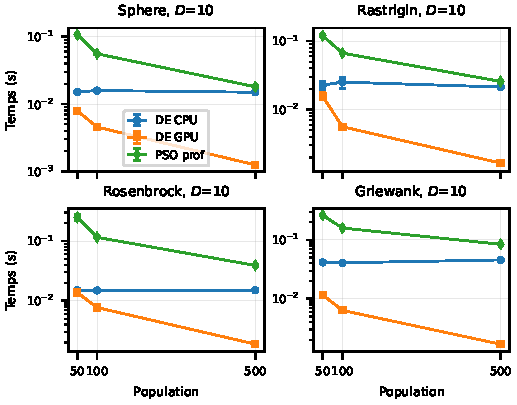
\includegraphics[width=\columnwidth]{figures/temps_d10.pdf}
\caption{Temps d'ex\'ecution moyen (\'echelle logarithmique) en fonction de la population, $D=10$ (barres : \'ecart-type sur 10 runs).}
\label{fig:temps10}
\end{figure}

\begin{figure}[!t]
\centering
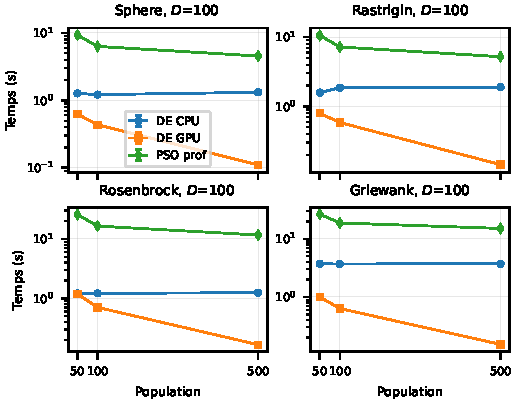
\includegraphics[width=\columnwidth]{figures/temps_d100.pdf}
\caption{Temps d'ex\'ecution moyen en fonction de la population, $D=100$.}
\label{fig:temps}
\end{figure}

\begin{table}[!t]\centering\scriptsize\setlength{\tabcolsep}{2pt}\caption{Sphere : EFV moyenne (10 runs ; plus petit = meilleur ; $1.2\mathrm{e}{-5}=1{,}2\times10^{-5}$).}\label{tab:sphere}
\begin{tabular}{rr|ccc}\toprule Dim & Pop & DE CPU & DE GPU & PSO prof\\\midrule
10 & 50 & 1.2e-5 & 1.1e-5 & 0.791\\
10 & 100 & 1.1e-5 & 9.9e-6 & 1.12\\
10 & 500 & 1.0e-5 & 1.1e-5 & 0.393\\
\midrule
50 & 50 & 1.4e-5 & 1.3e-5 & 46\\
50 & 100 & 1.3e-5 & 1.4e-5 & 33.9\\
50 & 500 & 0.174 & 0.208 & 37.1\\
\midrule
100 & 50 & 3.3e-5 & 2.5e-5 & 122\\
100 & 100 & 3.0e-5 & 3.7e-5 & 114\\
100 & 500 & 0.173 & 0.184 & 133\\
\bottomrule\end{tabular}\end{table}
\begin{table}[!t]\centering\scriptsize\setlength{\tabcolsep}{2pt}\caption{Rastrigin : EFV moyenne (10 runs ; plus petit = meilleur ; $1.2\mathrm{e}{-5}=1{,}2\times10^{-5}$).}\label{tab:rastrigin}
\begin{tabular}{rr|ccc}\toprule Dim & Pop & DE CPU & DE GPU & PSO prof\\\midrule
10 & 50 & 0.959 & 0.504 & 23.5\\
10 & 100 & 18.5 & 17.5 & 27.5\\
10 & 500 & 28.2 & 25.2 & 16.6\\
\midrule
50 & 50 & 30 & 33.5 & 382\\
50 & 100 & 173 & 243 & 331\\
50 & 500 & 420 & 421 & 325\\
\midrule
100 & 50 & 99.7 & 95.4 & 896\\
100 & 100 & 125 & 128 & 864\\
100 & 500 & 894 & 905 & 831\\
\bottomrule\end{tabular}\end{table}
\begin{table}[!t]\centering\scriptsize\setlength{\tabcolsep}{2pt}\caption{Rosenbrock : EFV moyenne (10 runs ; plus petit = meilleur ; $1.2\mathrm{e}{-5}=1{,}2\times10^{-5}$).}\label{tab:rosenbrock}
\begin{tabular}{rr|ccc}\toprule Dim & Pop & DE CPU & DE GPU & PSO prof\\\midrule
10 & 50 & 3.55 & 3.14 & 191\\
10 & 100 & 1.1e-5 & 1.0e-5 & 311\\
10 & 500 & 3.37 & 3.12 & 37.1\\
\midrule
50 & 50 & 56.5 & 46.9 & 4.5e4\\
50 & 100 & 20.4 & 20.7 & 2.5e4\\
50 & 500 & 175 & 164 & 2.8e4\\
\midrule
100 & 50 & 137 & 122 & 1.2e5\\
100 & 100 & 99.9 & 111 & 1.6e5\\
100 & 500 & 207 & 212 & 1.4e5\\
\bottomrule\end{tabular}\end{table}
\begin{table}[!t]\centering\scriptsize\setlength{\tabcolsep}{2pt}\caption{Griewank : EFV moyenne (10 runs ; plus petit = meilleur ; $1.2\mathrm{e}{-5}=1{,}2\times10^{-5}$).}\label{tab:griewank}
\begin{tabular}{rr|ccc}\toprule Dim & Pop & DE CPU & DE GPU & PSO prof\\\midrule
10 & 50 & 7.7e-3 & 0.0102 & 0.134\\
10 & 100 & 2.9e-3 & 5.5e-3 & 0.173\\
10 & 500 & 0.0324 & 0.033 & 0.0324\\
\midrule
50 & 50 & 6.7e-6 & 6.2e-6 & 0.839\\
50 & 100 & 7.0e-6 & 6.6e-6 & 0.618\\
50 & 500 & 5.5e-3 & 6.1e-3 & 0.701\\
\midrule
100 & 50 & 8.5e-6 & 7.5e-4 & 0.872\\
100 & 100 & 1.2e-5 & 1.8e-5 & 0.884\\
100 & 500 & 3.2e-3 & 3.5e-3 & 0.881\\
\bottomrule\end{tabular}\end{table}
\begin{table}[!t]\centering\scriptsize\setlength{\tabcolsep}{2pt}\caption{Temps moyen (s) sur les 4 fonctions (40 runs par case).}\label{tab:temps}
\begin{tabular}{rr|ccc}\toprule Dim & Pop & DE CPU & DE GPU & PSO prof\\\midrule
10 & 50 & 0.024 & 0.012 & 0.185\\
10 & 100 & 0.024 & 0.006 & 0.099\\
10 & 500 & 0.024 & 0.002 & 0.042\\
\midrule
50 & 50 & 0.478 & 0.389 & 4.567\\
50 & 100 & 0.499 & 0.222 & 3.071\\
50 & 500 & 0.502 & 0.052 & 2.092\\
\midrule
100 & 50 & 1.945 & 0.902 & 18.047\\
100 & 100 & 1.996 & 0.589 & 12.201\\
100 & 500 & 2.046 & 0.143 & 9.128\\
\bottomrule\end{tabular}\end{table}
\begin{table}[!t]\centering\scriptsize\setlength{\tabcolsep}{2pt}\caption{Taux de succ\`es, forme \emph{article / DE GPU $CR{=}0{,}9$ / DE GPU $CR{=}0{,}3$}. Article \cite{qin} : EFV $<10^{-8}$, 25 runs ; nos valeurs : EFV $<10^{-4}$, 10 runs.}\label{tab:sr}
\begin{tabular}{lr|ccc}\toprule Fonction & Dim & Pop 50 & Pop 100 & Pop 500\\\midrule
Sphere & 10 & 1.00/1.00/1.00 & 1.00/1.00/1.00 & 1.00/1.00/1.00\\
Sphere & 50 & 1.00/1.00/1.00 & 1.00/1.00/1.00 & 1.00/0.00/1.00\\
Sphere & 100 & 1.00/1.00/1.00 & 1.00/1.00/1.00 & 1.00/0.00/0.00\\
Rastrigin & 10 & 1.00/0.50/1.00 & 1.00/0.00/1.00 & 1.00/0.00/0.00\\
Rastrigin & 50 & 0.00/0.00/0.00 & 0.04/0.00/0.00 & 0.04/0.00/0.00\\
Rastrigin & 100 & 0.00/0.00/0.00 & 0.00/0.00/0.00 & 0.00/0.00/0.00\\
Rosenbrock & 10 & 0.44/0.00/0.00 & 0.32/1.00/0.00 & 0.00/0.00/0.00\\
Rosenbrock & 50 & 0.00/0.00/0.00 & 0.04/0.00/0.00 & 0.00/0.00/0.00\\
Rosenbrock & 100 & 0.00/0.00/0.00 & 0.00/0.00/0.00 & 0.00/0.00/0.00\\
Griewank & 10 & 1.00/0.20/0.90 & 1.00/0.80/1.00 & 1.00/0.00/0.00\\
Griewank & 50 & 0.92/1.00/1.00 & 1.00/1.00/1.00 & 1.00/0.00/1.00\\
Griewank & 100 & 0.84/0.90/1.00 & 0.96/1.00/1.00 & 0.96/0.00/1.00\\
\bottomrule\end{tabular}\end{table}
\begin{table}[!t]\centering\scriptsize\setlength{\tabcolsep}{2pt}\caption{DE GPU : EFV moyenne, forme \emph{$CR{=}0{,}9$ / $CR{=}0{,}3$} (10 runs).}\label{tab:cr}
\begin{tabular}{lr|ccc}\toprule Fonction & Dim & Pop 50 & Pop 100 & Pop 500\\\midrule
Sphere & 10 & 1.1e-5/1.2e-5 & 9.9e-6/1.1e-5 & 1.1e-5/1.2e-5\\
Sphere & 50 & 1.3e-5/3.9e-5 & 1.4e-5/4.2e-5 & 0.208/4.3e-5\\
Sphere & 100 & 2.5e-5/4.4e-5 & 3.7e-5/4.8e-5 & 0.184/5.0e-4\\
Rastrigin & 10 & 0.504/1.1e-5 & 17.5/1.1e-5 & 25.2/5.73\\
Rastrigin & 50 & 33.5/146 & 243/173 & 421/238\\
Rastrigin & 100 & 95.4/554 & 128/599 & 905/719\\
Rosenbrock & 10 & 3.14/2.65 & 1.0e-5/4.33 & 3.12/7.23\\
Rosenbrock & 50 & 46.9/38.1 & 20.7/40.3 & 164/47.2\\
Rosenbrock & 100 & 122/84.4 & 111/88.3 & 212/336\\
Griewank & 10 & 0.0102/7.5e-4 & 5.5e-3/6.2e-6 & 0.033/5.5e-4\\
Griewank & 50 & 6.2e-6/2.0e-5 & 6.6e-6/2.0e-5 & 6.1e-3/2.1e-5\\
Griewank & 100 & 7.5e-4/2.1e-5 & 1.8e-5/2.3e-5 & 3.5e-3/4.7e-5\\
\bottomrule\end{tabular}\end{table}
\begin{table}[!t]\centering\scriptsize\setlength{\tabcolsep}{2pt}\caption{Acc\'el\'eration $T_{\mathrm{CPU}}/T_{\mathrm{GPU}}$ du DE ($CR{=}0{,}9$).}\label{tab:speedup}
\begin{tabular}{lr|ccc}\toprule Fonction & Dim & Pop 50 & Pop 100 & Pop 500\\\midrule
Sphere & 10 & 1.9 & 3.5 & 12.0\\
Sphere & 50 & 0.8 & 1.4 & 6.1\\
Sphere & 100 & 2.0 & 2.8 & 11.9\\
Rastrigin & 10 & 1.5 & 4.5 & 12.9\\
Rastrigin & 50 & 1.7 & 3.0 & 13.7\\
Rastrigin & 100 & 2.0 & 3.2 & 13.2\\
Rosenbrock & 10 & 1.1 & 1.9 & 8.0\\
Rosenbrock & 50 & 0.5 & 0.9 & 3.7\\
Rosenbrock & 100 & 1.0 & 1.7 & 7.5\\
Griewank & 10 & 3.6 & 6.4 & 27.0\\
Griewank & 50 & 3.4 & 5.4 & 22.1\\
Griewank & 100 & 3.7 & 5.8 & 24.4\\
\bottomrule\end{tabular}\end{table}


%--------------------------------------------------------------
\section{Conclusion}
Nous avons transform\'e un PSO CUDA en DE/rand/1/bin, impl\'ement\'e en version s\'equentielle et en version GPU (un thread par individu), et compar\'e les deux au PSO d'origine sur quatre fonctions de test, trois dimensions et trois tailles de population. Le DE GPU est statistiquement \'equivalent au DE s\'equentiel en qualit\'e, jusqu'\`a 27 fois plus rapide, et nettement meilleur que le PSO de r\'ef\'erence \`a budget \'egal. Reprendre le param\`etre $CR=0{,}3$ de l'article am\'eliore nettement les grandes populations et Rastrigin $D{=}10$ et rapproche les taux de succ\`es de ceux de cudaDEi, mais d\'et\'eriore Rosenbrock ; l'effet d\'epend de la fonction.

Limites : (i) la fitness en simple pr\'ecision avec biais emp\^eche d'atteindre le seuil $10^{-8}$ de l'article ; (ii) avec un thread par individu, le GPU est peu utilis\'e pour de petites populations, et il peut \^etre plus lent que le CPU ; (iii) le PSO de r\'ef\'erence a \'et\'e gard\'e tel quel (avec la seule correction de Griewank), donc la comparaison n'est pas \`a son meilleur niveau ; (iv) pour l'am\'elioration du DE, nous n'avons test\'e que $CR=0{,}3$ (valeur de l'article), pas d'autres strat\'egies ni un r\'eglage de $F$ ou de $CR$ par fonction. Perspectives : \'evaluer la fitness en parall\`ele sur les dimensions, regrouper les noyaux avec la m\'emoire partag\'ee comme dans \cite{qin}, calculer en double pr\'ecision, et choisir $CR$ selon la fonction ou l'adapter en cours d'ex\'ecution (DE/best/1, param\`etres auto-adaptatifs).

%--------------------------------------------------------------
\begin{thebibliography}{3}
\bibitem{qin} A.~K. Qin, F.~Raimondo, F.~Forbes, and Y.~S. Ong, ``An improved CUDA-based implementation of differential evolution on GPU,'' in \emph{Proc. GECCO'12}, Philadelphia, USA, 2012.
\bibitem{storn} K.~Price, R.~Storn, and J.~Lampinen, \emph{Differential Evolution: A Practical Approach to Global Optimization}. Springer, 2005.
\bibitem{suganthan} P.~N. Suganthan \emph{et al.}, ``Problem definitions and evaluation criteria for the CEC 2005 special session on real-parameter optimization,'' Tech. Rep., Nanyang Technological University, 2005.
\end{thebibliography}

\end{document}
